\documentclass[a4paper, 10pt]{article}

\usepackage{graphicx}
\usepackage[T1]{fontenc}
\usepackage[polish]{babel}
\usepackage[utf8]{inputenc}
\usepackage{listings}
\usepackage{hyperref}
\usepackage{caption}
\usepackage{float}
\usepackage{xcolor}
\usepackage{color}
\usepackage[left=30mm, right=30mm, top=30mm, bottom=30mm]{geometry}


\graphicspath{{./figures}}

\renewcommand\contentsname{Spis treści}
\renewcommand\listfigurename{Spis rysunków}
\renewcommand\lstlistingname{Polecenie}
\renewcommand\lstlistlistingname{Spis poleceń}

\definecolor{codegreen}{rgb}{0,0.6,0}
\definecolor{codegray}{rgb}{0.5,0.5,0.5}
\definecolor{codepurple}{HTML}{C42043}
\definecolor{backcolour}{HTML}{F2F2F2}
\definecolor{bookColor}{cmyk}{0,0,0,0.90}
%\color{bookColor}

\captionsetup[lstlisting]{
    labelsep=period,
    justification=centering,
    singlelinecheck=false,
    width=0.9\linewidth
}

\captionsetup[figure]{
    justification=centering,
    singlelinecheck=false,
    width=.9\linewidth
}

\lstdefinestyle{SQL}{
    language=SQL,
    backgroundcolor=\color{backcolour},
    basicstyle=\footnotesize\ttfamily,
    breaklines=true,
    captionpos=b,
    commentstyle=\color{green},
    keywordstyle=\color{red},
    stringstyle=\color{red},
    showstringspaces=false,
    tabsize=2,
    morekeywords={USE, CREATE, TABLE, VARCHAR, INT, NOT, NULL, PRIMARY, KEY, AUTO_INCREMENT, INSERT, INTO, VALUES, SELECT, FROM, WHERE, ORDER, BY, ASC, DESC, GROUP, HAVING, UPDATE, SET, DELETE, JOIN, LEFT, RIGHT, OUTER, INNER, ON},
    frame=single,
    framesep=5pt,
    rulecolor=\color{gray},
    linewidth=1\linewidth
}

\begin{document}
\begin{titlepage}
\begin{center}
	
\includegraphics[scale=0.7]{logo.png}

	\vspace*{4cm}
	\textbf{Bazy danych\\ Laboratorium}

	\vspace{1.5cm}
	\textit{Wprowadzenie do Oracle}

	\vspace{1.5cm}
	\textbf{Stanislau Antanovich}\\
	nr. indeksu: 173590\\
	gr. lab: L04

	\vspace{4.5cm}
	\today
\end{center}
\end{titlepage}

\tableofcontents
\listoffigures
\lstlistoflistings

\newpage

\section{Wprowadzenie}
\subsection{Cel ćwiczenia}

Celem tego laboratorium jest zapoznanie się z narzędziem Oracle SQL Developer oraz praktyczne zastosowanie wiedzy na temat tworzenia, zarządzania i manipulowania bazami danych w Oracle. 

Poprzez realizację konkretnych zadań na przykładzie bazy danych ``Firma handlowa'', jest możliwość zdobycia umiejętności w obszarze tworzenia zapytań SQL, importowania i eksportowania danych, jak również zarządzania nimi przy użyciu interfejsu SQL Developer.

\subsection{Przygotowanie}

\begin{enumerate}
\item Zapoznanie się z narzędziem Oracle SQL Developer.
\item Przeanalizowanie struktury(tabele, pola, typy pól) pobranej bazy danych.
\item Zaimportowanie bazy danych ``Firma handlowa'' do narzędzia SQL Developer.
\end{enumerate}

\section{Realizacja}

Po zaimportowaniu bazy danych ``Firma handlowa'' do narzędzia SQL developer można zaczynać wykonywać polecenia SQL.

\begin{enumerate}

\item Wyświetlienie wszystkiej informacji o pracownikach
\begin{lstlisting}[style=SQL, caption=\textit{Wyświetlenie informacji o pracownikach}]
SELECT * FROM PRACOWNICY;
\end{lstlisting}

\begin{figure}[H]
	\centering
	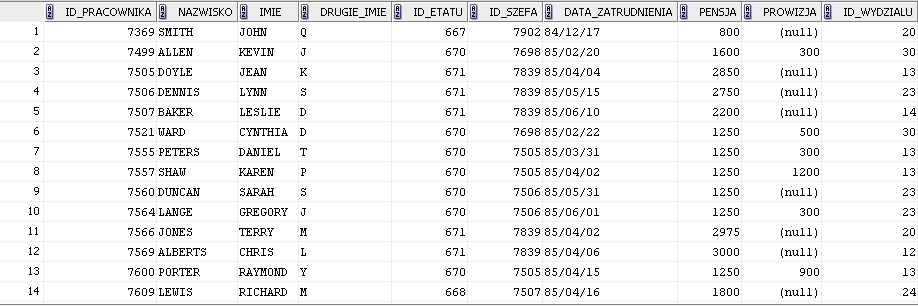
\includegraphics[scale=0.7]{zadanie1.png}
	\caption{\textit{Wyświetlenie informacji o pracownikach}}
	\label{fig:wszystko}
\end{figure}

\item Wyświetlienie informacji o imieniu, nazwisku i pensji pracowników
\begin{lstlisting}[style=SQL, caption=\textit{Wyświetlienie informacji o imieniu, nazwisku i pensji pracowników}]
SELECT IMIE,NAZWISKO,PENSJA FROM PRACOWNICY;
\end{lstlisting}

\begin{figure}[H]
	\centering
	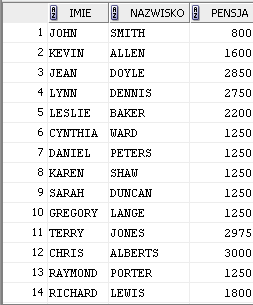
\includegraphics[scale=0.7]{zadanie2.png}
	\caption{\textit{Wyświetlienie informacji o imieniu, nazwisku i pensji pracowników}}
	\label{fig:imie_nazwisko_pensja}
\end{figure}

\item Wypisywanie wszystkich Pracowników, sortując na podstawie Nazwiska w kolejności przeciwnej do alfabetycznej
\begin{lstlisting}[style=SQL, caption=\textit{Wypisywanie wszystkich Pracowników, sortując na podstawie Nazwiska w kolejności przeciwnej do alfabetycznej}]
SELECT * FROM PRACOWNICY ORDER BY NAZWISKO DESC;
\end{lstlisting}

\begin{figure}[H]
	\centering
	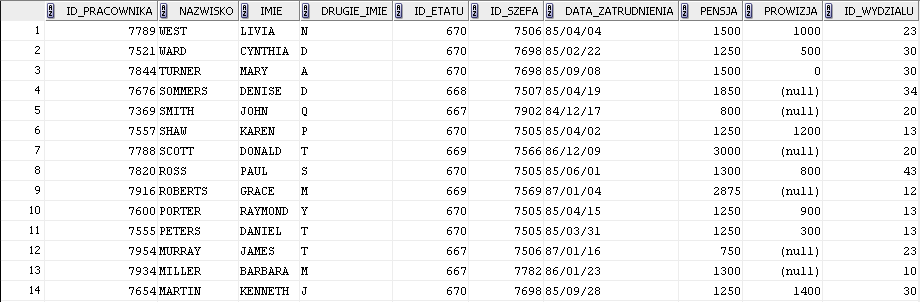
\includegraphics[scale=0.7]{zadanie3.png}
	\caption{\textit{Wypisywanie wszystkich Pracowników, sortując na podstawie Nazwiska w kolejności przeciwnej do alfabetycznej}}
	\label{fig:nazwisko_sort_desc}
\end{figure}

\item Wyświetlienie informacji o imieniu, nazwisku i pensji pracowników, których pensja jest > 1500
\begin{lstlisting}[style=SQL, caption=\textit{Wyświetlienie informacji o imieniu, nazwisku i pensji pracowników, których pensja jest > 1500}]
SELECT IMIE,NAZWISKO,PENSJA FROM PRACOWNICY WHERE PENSJA > 1500;
\end{lstlisting}

\begin{figure}[H]
	\centering
	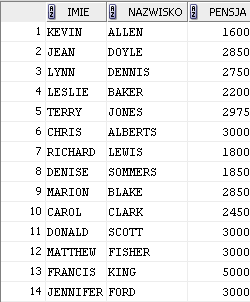
\includegraphics[scale=0.7]{zadanie4.png}
	\caption{\textit{Wyświetlienie informacji o imieniu, nazwisku i pensji pracowników, których pensja jest > 1500}}
	\label{fig:pensja_1500}
\end{figure}


\item Wyświetlienie zamówień o wartości z przedziału <1000,3000>, złożonych po dniu 10-05-1991
\begin{lstlisting}[style=SQL, caption=\textit{Wyświetlienie zamówień o wartości z przedziału <1000,3000>, złożonych po dniu 10-05-1991}]
SELECT * FROM ZAMOWIENIA WHERE WARTOSC BETWEEN 1000 AND 3000 AND DATA_ZAMOWIENIA > '91/05/10';
\end{lstlisting}

\begin{figure}[H]
	\centering
	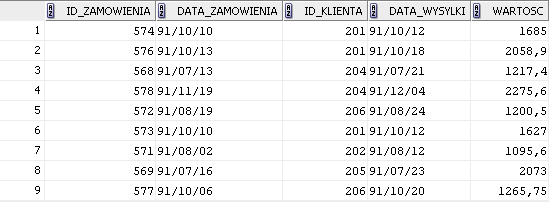
\includegraphics[scale=0.7]{zadanie5.png}
	\caption{\textit{Wyświetlienie zamówień o wartości z przedziału <1000,3000>, złożonych po dniu 10-05-1991}}
	\label{fig:zamowienia_data}

\end{figure}


\item Sortowanie wyniku zadania 5 po datach złożenia zamówień i po wartościach zamówień
\begin{lstlisting}[style=SQL, caption=\textit{Sortowanie wyniku zadania 5 po datach złożenia zamówień i po wartościach zamówień}]
SELECT * FROM ZAMOWIENIA WHERE WARTOSC BETWEEN 1000 AND 3000 AND DATA_ZAMOWIENIA > '91/05/10' ORDER BY DATA_ZAMOWIENIA,WARTOSC;
\end{lstlisting} 

\begin{figure}[H]
	\centering 
	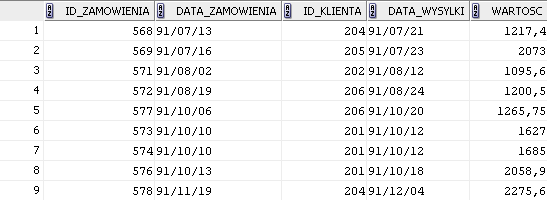
\includegraphics[scale=0.7]{zadanie6.png}
	\caption{\textit{Sortowanie wyniku zadania 5 po datach złożenia zamówień     i po wartościach zamówień}}
	\label{fig:zamowienia_data_sort}
\end{figure}

\item Dodawanie pracownika o danych z przykładowymi wartościami
\begin{lstlisting}[style=SQL,caption=\textit{Dodawanie pracownika o danych z przykładowymi wartościami}]
INSERT INTO PRACOWNICY VALUES (7999,'ATANOVICH','STANISLAU','S',667,7506,TO_DATE(2446812,'J'),750,NULL,23);
\end{lstlisting}

\begin{figure}[H]
	\centering 
	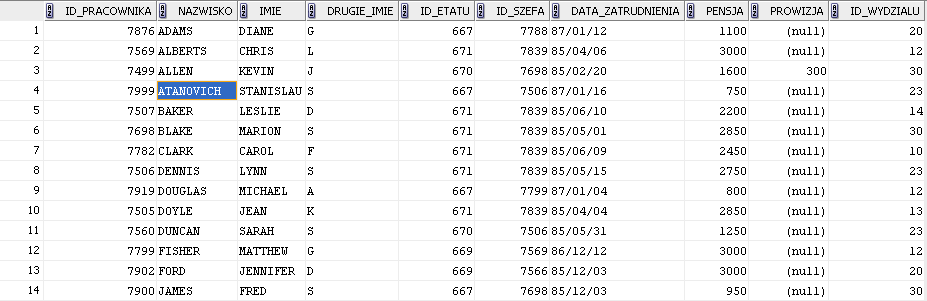
\includegraphics[scale=0.7]{zadanie7.png}
	\caption{\textit{Dodawanie pracownika o danych z przykładowymi wartościami}}
	\label{fig:dodawanie_pracownika}
\end{figure}

\item Modyfikacja płacę dodanego pracownika do wartości 2000. 
\begin{lstlisting}[style=SQL, caption=\textit{Modyfikacja płacę dodanego pracownika do wartości 2000}]
UPDATE PRACOWNICY SET PENSJA = 2000 WHERE IMIE = 'STANISLAU' AND NAZWISKO = 'ATANOVICH';
\end{lstlisting}

\begin{figure}[H]
	\centering 
	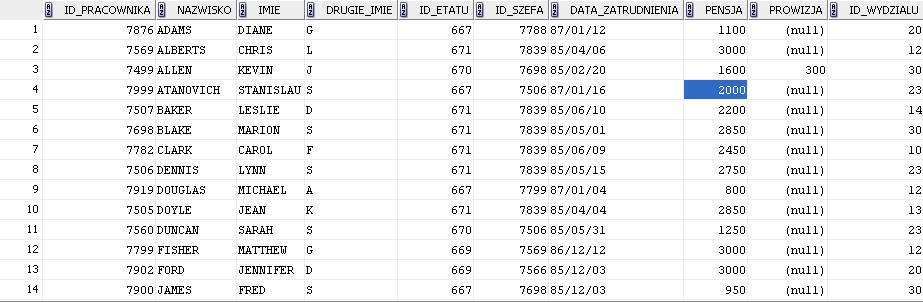
\includegraphics[scale=0.7]{zadanie8.png}
	\caption{\textit{Modyfikacja płacę dodanego pracownika do wartości 2000}}
	\label{fig:modyfikacja_pracownika}
\end{figure}

\item Usunięcie dodanego pracownika w podpunkcie. 
\begin{lstlisting}[style=SQL, caption=\textit{Usunięcie dodanego pracownika}]
DELETE FROM PRACOWNICY WHERE NAZWISKO = 'ATANOVICH' AND IMIE = 'STANISLAU';
\end{lstlisting}

\begin{figure}[H]
	\centering 
	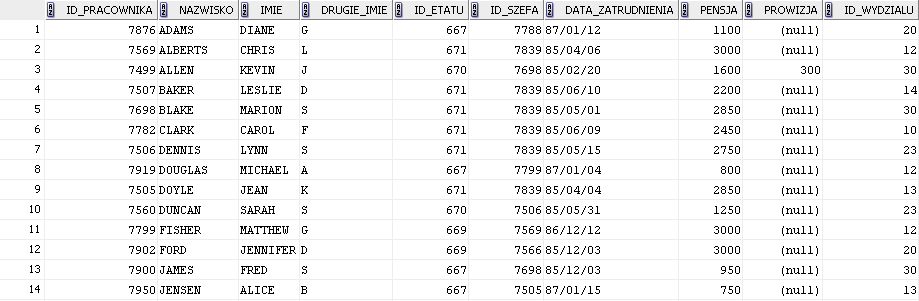
\includegraphics[scale=0.7]{zadanie9.png}
	\caption{\textit{Usunięcie dodanego pracownika}}
	\label{fig:usuniecie_pracownika}
\end{figure}

\item Wyświetlienie imia i nazwiska i nazwę etatu pracowników zatrudnionych na etacie ANALYST. Wybieranie danych z dwóch tabel, należy zastosować złączenie (odpowiedni warunek w WHERE lub klauzulę JOIN).
\begin{lstlisting}[style=SQL, caption=\textit{Wyświetlienie imia i nazwiska i nazwę etatu pracowników zatrudnionych na etacie ANALYST}]
SELECT PRACOWNICY.IMIE,PRACOWNICY.NAZWISKO,ETATY.ETAT FROM PRACOWNICY JOIN ETATY ON ETATY.ID_ETATU = PRACOWNICY.ID_ETATU WHERE ETATY.ETAT = 'ANALYST';
\end{lstlisting}

\begin{figure}[H]
	\centering 
	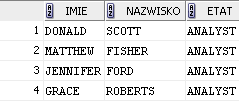
\includegraphics[scale=0.7]{zadanie10.png}
	\caption{\textit{Wyświetlienie imia i nazwiska i nazwę etatu pracowników zatrudnionych na etacie ANALYST}}
	\label{fig:join_etat_analyst}
\end{figure}

\item Wyświetlienie wszystkich pracowników na etacie MANAGER, wynik posortowany po identyfikatorze.
\begin{lstlisting}[style=SQL, caption=\textit{Wyświetlienie wszystkich pracowników na etacie MANAGER, wynik posortowany po identyfikatorze}]
SELECT PRACOWNICY.IMIE,PRACOWNICY.NAZWISKO,ETATY.ETAT FROM PRACOWNICY JOIN ETATY ON ETATY.ID_ETATU = PRACOWNICY.ID_ETATU WHERE ETATY.ETAT = 'MANAGER' ORDER BY PRACOWNICY.ID_PRACOWNIKA;
\end{lstlisting}

\begin{figure}[H]
	\centering 
	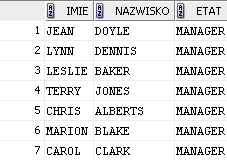
\includegraphics[scale=0.7]{zadanie11.png}
	\caption{\textit{Wyświetlienie wszystkich pracowników na etacie MANAGER, wynik posortowany po identyfikatorze}}
	\label{fig:join_etat_manager}
\end{figure}
\end{enumerate}

\section{Wnioski}

Podczas tego zajęcia laboratoryjnego nauczyłem się wielu ważnych rzeczy związanych z wykorzystaniem narzędzia ``SQL Developer'' do pracy z bazami danych.

Podczas wykonania zadań stosowałem różne rodzaje zapytań SQL, takie jak zapytania proste o wyświetlanie danych, sortowanie, filtrowanie, łączenie tabel, dodawanie, modyfikowanie i usuwanie rekordów.

Poprzez wykonywanie różnych zapytań SQL na bazie danych pracowników, lepiej zrozumiałem strukturę bazy danych. W trakcie wykonania zadań używałem następujące warunki: \textbf{WHERE, ORDER BY ASC/DESC, JOIN}. Te warunki pozwoliły mi na lepsze zrozumienie jak efektywnie wybierać dane z tablic.


\end{document}
